\section{Лекция номер 7}

\subsection{Функциональные последовательности}

\begin{conj}
    Поточечная сходимость.

    Пусть $f_n, f: E \to \R$. 
    Тогда говорят, что $f_n$ пототечно сходится к $f$, если \[ \forall x \in E \; \lim_{n \to +\infty} f_n(x) = f(x) \]
    Обозначение: $f_n \to f$,  где $f$ -- предельная функция.
\end{conj}

То есть смысл такой, что мы фиксируем конкретный $x_0$, подставляем его во все функции, получаем обычную числовую последовательность, находим ее предел и говорим,
что это $f(x_0)$.
Проделываем это для всех $x_0 \in E$ и получаем $f$, заданную на $E$.

\vspace*{5mm}

\begin{conj}
    Равномерная сходимость.

    Пусть $f_n, f: E \to \R$.
    Тогда говорят, что $f_n$ равномерно сходится к $f$ на $E$, если \[ \forall \; \varepsilon > 0 \; \exists N: \; \forall n \geqslant N \; \forall x \in E \; \abs{f_n(x) - f(x)} < \varepsilon \]
    Обозначение: $f_n \doublerightarrow f$.
\end{conj}

\vspace*{5mm}

На первый взгляд определения очень похожи.
Чтобы заметить отличия, давайте запишем определение поточечной сходимости с кванторами: \[ \forall x \in E \; \forall \varepsilon > 0 \; \exists N: \forall n \geqslant N \; \abs{f_n(x) - f(x)} < \varepsilon \]
Теперь видим, что в определении поточечной сходимости $N$ выбирается для каждого $x \in E$ по отдельности, 
в то время как в определении равномерной сходимости выбирается универсальное $N$, подходящее для всех $x \in E$.

Заметим, что условие равномерной сходиомсти более сильное, и в частности, $f_n \doublerightarrow f \Longrightarrow f_n \to f$.
Приведем пример, показывающий, что обратной стрелки у нас нет.

\vspace*{5mm}

\begin{example}
    $E = (0, 1), \, f_n(x) = x^n, \, f_n \to f \equiv 0$ (при подстановке каждого $x$ в пределе получаем 0)

Запишем определение равномерной сходимости:
\[ \forall \varepsilon > 0 \; \exists N: \; \forall n \geqslant N \; \forall x \in (0, 1): \; x^n < \varepsilon \]
\end{example}
Понятно, что это нерправда, ведь зафиксировав конкретный $\varepsilon < 1$ и конкретный $N$, для любого $n \geqslant N$ мы всегда сможем найти такой $x$ близкий к 1, что $x^n \geqslant \varepsilon$.
Таким образом, равномерной сходимости нет.

\vspace*{7mm}

\textbf{Поясняющая картинка к равномерной сходимости}.

Пусть $f_n \rightrightarrows f$. 
Тогда условие \[ \forall \; \varepsilon > 0 \; \exists N: \; \forall n \geqslant N \; \forall x \in E \; \abs{f_n(x) - f(x)} < \varepsilon \] 
означает, что для любого $\varepsilon > 0$ найдется такой достаточно большой номер $N$, что, начиная с него, графики всех функций $f_n(x)$ будут лежать в полоске шириной $2\varepsilon$ относительно графика $f(x)$:
\begin{center}
    %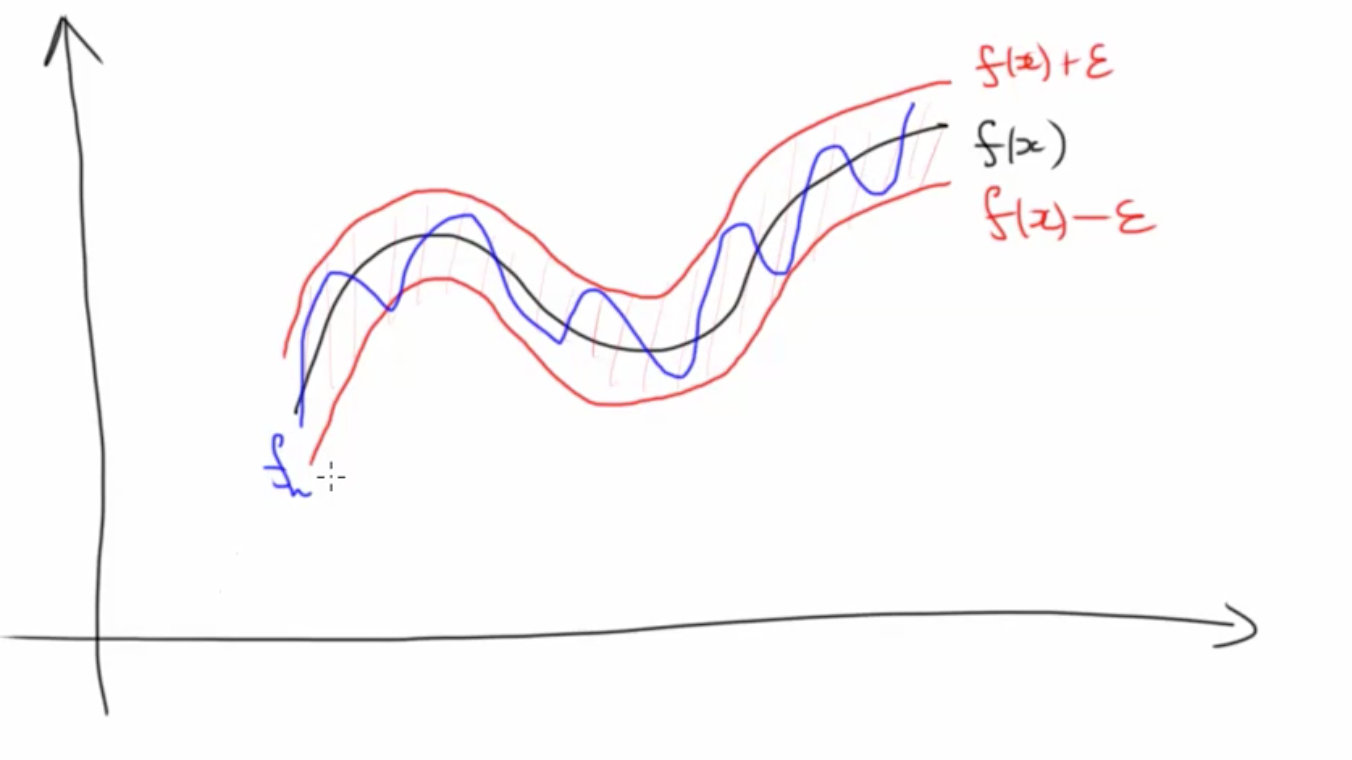
\includegraphics[scale=0.5]{Uniform_convergence.png} 
    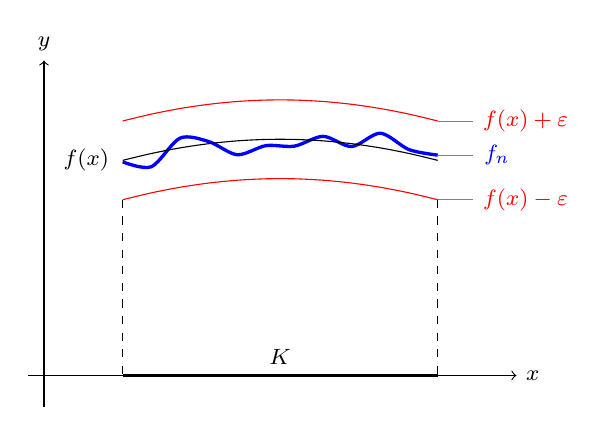
\begin{tikzpicture}[auto,
        B/.style = {decorate,
                    decoration={brace, amplitude=3pt,
                    pre=moveto,pre length=1pt,post=moveto,post length=1pt,
                    raise=1mm}},
           domain = -30:30, samples=12, smooth,
             font = \footnotesize
                                ]
        % coordinates
        \draw[->] (-0.2,0) -- (6,0) node[right]{$x$};
        \draw[->] (0,-0.4) -- (0,4) node[above]{$y$};
        % curve
        \draw[very thick, blue] 
            plot ({(45+\x)/15},{1+rand/5+2*cos(\x)})
            node[coordinate,pin=0:$f_n$] {};
        % convergence borders
        \draw[red]  plot ({(45+\x)/15},{1.5+2*cos(\x)}) 
                    node[coordinate,pin=0:$f(x)+\varepsilon$] {};
        \draw[black] plot ({(45+\x)/15},{1.0+2*cos(\x)}) coordinate (e2);
        \draw[red]  plot ({(45+\x)/15},{0.5+2*cos(\x)}) 
                    node[coordinate,pin=0:$f(x)-\varepsilon$] {};
    
        % labels on the left side
        \draw (1,{1.75+cos(-10)}) node[left=0.5mm]   {$f(x)$} ++ (0,1);
        \draw[dashed]   (1,{0.5+2*cos(30)}) -- (1,0)
                        (5,{0.5+2*cos(30)}) -- (5,0);
    
        \draw[very thick]    (1,0) -- node[above] {$K$} (5,0);
        
    \end{tikzpicture}   
\end{center}

\vspace*{10mm}

\begin{conj}
    Равномерно ограниченная последовательность.

    $f_n: E \to \R$~--- равномерно ограниченная последовательность, если
    \[ \exists \; M: \; \forall x \in E, \; \forall n \in \N: \; |f_n(x)| \leqslant M \]
\end{conj}

\vspace*{5mm}

Мы можем задать эквивалентное определение равномерной сходимости, которое на практике иногда оказывается чуть более удобным, 
хотя по сути это просто переформулировка изначального.

\begin{theorem}
    $f_n \doublerightarrow f$ на $E \Longleftrightarrow \sup\limits_{x \in E}{\abs{f_n(x) - f(x)}} \to 0$
\end{theorem}

\newpage

\begin{proof} \quad

    "$\Longrightarrow$":
    \begin{gather*}
        \begin{split}
            f_n \doublerightarrow f \text{ на } E &\Longleftrightarrow \forall \varepsilon > 0 \;\; \exists N \;\; \forall n \geqslant N \;\; \forall x \in E: \; \abs{f_n(x) - f(x)} < \varepsilon \\
            &\Longrightarrow \varepsilon - \text{ верхняя граница для } \abs{f_n(x) - f(x)} \\
            &\Longrightarrow \sup_{x \in E}{\abs{f_n(x) - f(x)}} \leqslant \varepsilon \\
            &\Longrightarrow \forall \varepsilon > 0 \;\; \exists N: \; \forall n \geqslant N \; \sup_{x \in E}{\abs{f_n(x) - f(x)}} \leqslant \varepsilon \\
            &\Longleftrightarrow \sup_{x \in E}{\abs{f_n(x) - f(x)}} \to 0
        \end{split}
    \end{gather*}

    "$\Longleftarrow$":
    \begin{gather*}
        \begin{split}
            \sup_{x \in E}{\abs{f_n(x) - f(x)}} \to 0 &\Longleftrightarrow \forall \varepsilon > 0 \; \exists N: \; \forall n \geqslant N \; \sup_{x \in E}{\abs{f_n(x) - f(x)}} < \varepsilon \\
            &\Longrightarrow \forall \varepsilon > 0 \; \exists N: \forall n \geqslant N \; \forall x \in E :\; \abs{f_n(x) - f(x)} < \varepsilon
        \end{split}
    \end{gather*}
\end{proof}

\follow

\begin{enumerate}
    \item $\abs{f_n(x) - f(x)} \leqslant a_n \; \forall x \in E$ и $a_n \to 0$, то $f_n \doublerightarrow f$ на $E$
    \begin{proof}
        $\abs{f_n(x) - f(x)} \leqslant a_n \Longrightarrow \sup\limits_{x \in E}{\abs{f_n(x) - f(x)}} \leqslant a_n \to 0$
    \end{proof}
    \item $f_n \not \doublerightarrow f$ на $E$ $\Longleftrightarrow \exists x_n \in E$, т.ч. $f_n(x_n) - f(x_n) \not \to 0$
    \begin{proof} \quad 

        \quad "$\Longleftarrow$": $\;\; \sup\limits_{x \in E}{\abs{f_n(x) - f(x)}} \geqslant \abs{f_n(x_n) - f(x_n)} \not \to 0 \Longrightarrow \sup\limits_{x \in E}{\abs{f_n(x) - f(x)}} \not \to 0$

        \quad "$\Longrightarrow$": $\;\; f_n \not \doublerightarrow f \Longrightarrow \sup\limits_{x \in E}{\abs{f_n(x) - f(x)}} \not \to 0 \Longrightarrow$ легко можно выбрать такую $x_n$, что $f_n(x_n) - f(x_n) \not \to 0$
    \end{proof}
    Мы получили условие на отсутствие равномерной сходимости.
    Применим его в нашем предыдущем примере: \[ f_n(x) = x^n \Rightarrow \forall n \; \sup_{x \in (0, 1)}{x^n} = 1 \not \to 0 \Rightarrow f_n  \not \doublerightarrow 0   \]
\end{enumerate}

\vspace*{5mm}

\begin{theorem}
    Если $f_n$ равномерно ограничена и $g_n \doublerightarrow 0$, то $f_n \cdot g_n \doublerightarrow 0$.
\end{theorem}
\begin{proof}
    Распишем равномерную ограниченность: $\forall n \in \N  \; \forall x \;\; \abs{f_n(x)} \leqslant M$.

    Надо доказать, что $\sup\limits_{x \in E}{\abs{f_n(x)g_n(x)}} \to 0$:
    \[ \abs{f_n(x) \cdot g_n(x)} \leqslant M \cdot \abs{g_n(x)} \Longrightarrow \sup_{x \in E}{\abs{f_n(x) - f(x)}} \leqslant M \cdot \sup_{x \in E}{\abs{g_n(x)}} \to 0 \]
\end{proof}

\begin{theorem}[Критерий Коши] 
    Пусть $f_n: E \to \R$. Тогда
    \[ f_n - \text{ равномерно сходится } \Longleftrightarrow \forall \varepsilon > 0 \; \exists N \; \forall n,m \geqslant N: \; \forall x \in E \; \abs{f_n(x) - f_m(x)} < \varepsilon \]
\end{theorem}

\begin{proof} \quad

    "$\Longrightarrow$":
    \begin{gather*}
        \begin{split}
            f_n \doublerightarrow f &\Longrightarrow \forall \varepsilon > 0 \;\; \exists N \;\; \forall n \geqslant N \;\; \forall x \in E: \; \abs{f_n(x) - f(x)} < \frac{\varepsilon}{2} \\
            &\Longrightarrow \forall n, m \geqslant N \; \forall x \in E: \begin{cases}
                \abs{f_n(x) - f(x)} < \frac{\varepsilon}{2} \\
                \abs{f_m(x) - f(x)} < \frac{\varepsilon}{2} 
            \end{cases} \\
            &\Longrightarrow  \abs{f_n(x) - f_m(x)} \leqslant \abs{f_n(x) - f(x)} + \abs{f(x) - f_m(x)} < \varepsilon \\
        \end{split}
    \end{gather*}

    "$\Longleftarrow$": Зафиксируем $x_0 \in E$. 
    Тогда их условия $\forall \varepsilon > 0 \; \exists N: \forall n, m \geqslant N \; \abs{f_n(x_0) - f_m(x_0)} < \varepsilon$ будет следовать, что $f_n(x_0)$ -- 
    фундаментальная последовательность.
    Согласно критерию Коши для числовой последовательности существует конечный $\lim\limits_{n \to +\infty} f_n(x_0) =: f(x_0)$.
    Проделаем это для всех $x \in E$. 
    Осталось доказать, что $f_n \doublerightarrow f$:

    \[ \forall \varepsilon > 0 \; \exists N: \; \forall n, m \geqslant N \; \forall x \in E \; \abs{f_n(x) - f_m(x)} < \varepsilon \stackrel{m \to +\infty}{\Longrightarrow} \abs{f_n(x) - f(x)} \leqslant \varepsilon \Longrightarrow f_n \doublerightarrow f \]


\end{proof}

\begin{conj} Нормированое пространство ограниченных функций
    \[ l^{\infty}(E) := \{ f: E \to R; f - \text{ ограниченая функция} \} \]
    
    Введем на этом пространстве следующую норму:    
    \[ \norm{f}_{l^{\infty}(E)} := \norm{f}_{\infty} := \sup_{x \in E}{\abs{f(x)}} \text{ (он конечен, т.к. $f$~--- ограничена)} \]

    Аксиомы нормы очевидны (кроме неравенства $\triangle$):
    \begin{gather*}
        \norm{f + g}_{\infty} \leqslant \norm{f}_{\infty} + \norm{g}_{\infty} \\
        \sup_{x \in E}{\abs{f(x) + g(x)}} \leqslant \sup_{x \in E}(\abs{f(x)} + \abs{g(x)}) \leqslant \sup_{x \in E}{\abs{f(x)}} + \sup_{x \in E}{\abs{g(x)}} = \norm{f}_{\infty} + \norm{g}_{\infty}
    \end{gather*}
\end{conj}

\vspace*{5mm}

\notice \;
Равномерная сходимость $=$ сходимость по норме $\norm{\cdot}_{l^{\infty}(E)}$:
\[ f_n \doublerightarrow f \text{ на } E \Longleftrightarrow \norm{f_n - f}_{l^{\infty}(E)} \to 0 \]
Это действительно так, ведь просто по определению $\norm{f_n - f}_{l^{\infty}(E)} = \sup_{x \in E}{\abs{f_n(x) - f(x)}}$)

\newpage

\begin{theorem}
    $l^{\infty}(E)$~--- полное пространство.
\end{theorem}

\begin{proof}
    Нужно доказать, что любая фундаментальная последовательность имеет предел, лежащий в этом пространстве.

    \quad Пусть $f_n$~--- фундаментальная последовательность:
    \begin{gather*}
        \forall \varepsilon > 0 \; \exists N: \; \forall n,m \geqslant N \;\; \underbrace{\norm{f_n(x) - f_m(x)}}_{= \sup\limits_{x \in E}{\abs{f_n(x) - f(x)}}} < \varepsilon \\
        \Longrightarrow \forall \varepsilon > 0 \;\; \exists N: \forall n,m \geqslant N \;\; \forall x \in E \;\;\;\; \abs{f_n(x) - f_m(x)} < \varepsilon - \text{ это критерий Коши} \\
        \Longrightarrow f_n \doublerightarrow f \Longrightarrow \norm{f_n - f} \to 0
    \end{gather*}
    \quad Осталось убедиться, что $f$, к которой сходится наша фундоментальная последовательность, лежит в нашем пространстве, т.е. является ограниченной функцией.

    \quad Возьмём $\varepsilon = 1$ из определения предела: $\; \exists N \; \forall n \geqslant N \;\; \norm{f_n - f} < 1$. 
    В терминах супремума это означает, что $\sup\limits_{x \in E}{\abs{f_n(x) - f(x)}} < 1$.
    Оставим только $N$-тую функцию: $\forall x \in E \;\; \abs{f_{N}(x) - f(x)} < 1$.
    Мы знаем, что она ограничена, так как лежит в $l^{\infty}(E)$, поэтому $\forall x \in E \;\; \abs{f(x)} < 1 + \abs{f_{N}(x)} \leqslant 1 + C$.
\end{proof}

\vspace*{5mm}

У равномерной сходимости есть много полезных свойств.
Одно их них заключается в том, что при равномерной сходимости сохраняется непрерывность.

\begin{theorem}
    Пусть $f_n: E \to \R$ непрерывны в $(\cdot) \, a \in E$ и $f_n \doublerightarrow f$ на $E$. 
    Тогда $f$ непрерывна в $(\cdot) \, a$.
\end{theorem}
\begin{proof}
    Зафиксируем $\varepsilon > 0$. 
    Распишем равномерную сходимость:
    $\exists N \; \forall n \geqslant N: \; \forall x \in E \;\; \abs{f_n(x) - f(x)} < \varepsilon$.
    Оставим только $N$-тую функцию: $\forall x \in E \;\; \abs{f_N(x) - f(x)} < \varepsilon$.
    Напишем следующее неравенство треугольника $\forall x \in E$:
    \[ \abs{f(x) - f(a)} \leqslant \underbrace{\abs{f(x) - f_N(x)}}_{< \varepsilon} + \abs{f_N(x) - f_N(a)} + \underbrace{\abs{f_N(a) - f(a)}}_{< \varepsilon} < 2\varepsilon + \abs{f_N(x) - f_N(a)} \]
    \quad Для оценки $\abs{f_N(x) - f_N(a)}$ воспользуемся непрерывностью $f_N$ в $(\cdot) \, a$: 
    \[ \exists \delta > 0: \; \forall x \in E: \; \abs{x - a} < \delta \;\;\; \abs{f_N(x) - f_N(a)} < \varepsilon \]
    \quad Таким образом, мы взяли произвольный $\varepsilon$ и смогли подобрать такое $\delta$, что если $\abs{x - a} < \delta$, то $\abs{f(x) - f(a)} < 3\varepsilon$.
    Это и есть критерий непрерывности $f$ в $(\cdot) \, a$.
\end{proof}

\vspace*{4mm}

\follow (т. Стокса-Зайделя)

Если $f_n \in C(E)$ -- непрерывны на $E$ и $f_n \doublerightarrow f$ на $E$, то $f \in C(E)$.
Действительно, в каждой точке непрерывность сохраняется, поэтому сохраняется и общая непрерывность.

\vspace*{4mm}

\notice \, Поточечной сходимости не хватает для сохранения непрерывности.

Разберем пример: $f_n(x) = x^n : [0, 1] \to \R, f(x) = \begin{cases} 
    1, & \text{если } x = 1 \\ 
    0, & \text{иначе} x \in [0, 1) 
\end{cases}$

$f_n(x) \ C[0, 1]$, а вот предельная функция непрерывной не является.

\vspace*{7mm}

\begin{conj}
    Нормированное пространство непрерывных функций.
    \[ C(K) := \{ f: K \to \R; f - \text{ непрерывна} \}, \text{ где } K - \text{ компакт } \]

    Введем на этом пространстве следующую норму:
    \[ \norm{f}_{C(K)} := \max_{x \in K}{\abs{f(x)}} = \sup_{x \in K}{\abs{f(x)}} \] 

    Заметим, что $C(K)\subset l^{\infty}(K)$, так как функция, непрерывная на компакте, ограничена, и нормы у этих пространств совпадают.
\end{conj}

\vspace*{5mm}

\textbf{\textit{Следствие}} (из т. Стокса-Зайделя):
$C(K)$~--- замкнутое подпространство $l^{\infty}(K)$.

\begin{proof}
    Берём $f_n \in C(K)$ и $\norm{f_n - f} \to 0$.
    Надо доказать, что $f \in C(K)$.
    Это прямое следствие теоремы Стокса-Зайделя, ведь $\norm{f_n - f} \to 0 \Leftrightarrow f_n \doublerightarrow f$.
\end{proof}

\vspace*{5mm}

Логично предположить, что $C(K)$ аналогично $l^{\infty}(K)$ будет полным пространством.
Чтобы доказать это, сформулируем чуть более общую теорему.

\begin{theorem}
    Замкнутное подпространство полного пространства -- полное пространство.
\end{theorem}
\begin{proof}
    Пусть $X$ -- полное пространство, а $Y$ -- замкнутое подпространство в $X$.
    Возьмём фундаментальную последовательность в $Y: a_n \in Y \Longrightarrow a_n$ -- фундаментальна в $X$.
    Воспользоваашись полнтой $X$, заключаем, что $\lim a_n =  a \in X$.
    А так как $Y$ замкнутое, $a$ будет лежать в $Y$, поэтому $Y$ -- полное.
\end{proof}

\follow \; $C(K)$~--- полное нормированное пространство.

\subsection{Функциональные ряды}
\begin{conj}
    $\sum\limits_{n = 1}^\infty u_n(x)$, где $u_n: E \to \R$ -- функциональный ряд.    
\end{conj} 
Аналогично обычным рядам можно ввести частичную сумму: $S_n(x) := \sum\limits_{k = 1}^n u_k(x)$.
То есть мы берем и честно суммируем первые $n$ функций и в итоге получаем функцию $S_n(x)$.
\begin{conj}
    Ряд сходится поточечно, если последовательность $S_n(x)$ сходятся поточечно.
    Можно переформулировать это так: ряд сходится поточечно, если для любого $x \in E$ соотвествующий числовой ряд будет сходящимся.

    Поточечно сходящийся ряд определяет новую функцию $S(x): E \to \R \;\; S(x) = \sum\limits_{n = 1}^\infty u_n(x)$.
    Тогда можно определить остаток ряда $r_n(x) := \sum\limits_{k = n + 1}^\infty u_k(x) = S(x) - S_n(x)$.
\end{conj}

\vspace*{5mm}

\begin{conj}
    Ряд сходится равномерно, если $S_n$ сходятся равномерно на $E$.
\end{conj}

\begin{theorem}
    Ряд $\sum\limits_{n = 1}^\infty u_n(x)$ равномерно сходится $\Longleftrightarrow r_n \doublerightarrow 0$. 
\end{theorem}
\begin{proof}
    Если ряд равномерно сходится, то по определению $S_n \doublerightarrow S$.
    Вычтем из обоих частей $S$ и получим, что $S_n - S \doublerightarrow 0$.
    Таким образом, $-r_n \doublerightarrow 0$, что эквивалентно $r_n \doublerightarrow 0$.
\end{proof}

\vspace*{5mm}

\textbf{Необходимое условие равномерной сходимости.} Если ряд $\sum\limits_{n = 1}^\infty u_n(x)$ сходится равномерно, то $u_n \doublerightarrow 0$.
Доказательство аналогично числовым рядам: $S_n \doublerightarrow S \Rightarrow u_n = S_n - S_{n-1} \doublerightarrow S - S = 0$.
Если взять отрицание этого условия, то получится, что если найдется такая последовательность $x_n$, что $u_n(x_n) \nrightarrow 0$, то $\sum\limits_{n = 1}^\infty u_n(x)$ не является равномерно сходящимся.
    
\notice \, Из расходимости ряда $\sum\limits_{n = 1}^\infty u_n(x_n)$ ничего не следует.
То есть мы не можем подставить в каждую функцию свой плохой аргумент, получить расходящийся ряд и сказать, что равномерной сходимости нет.
Это иллюстрирует следующий пример.

\begin{example}
    $u_n(x) = \begin{cases}
        \frac{1}{n}, & \text{при }x \in [\frac{1}{n + 1}, \frac{1}{n}) \\
        0, & \text{иначе}
    \end{cases}$
    \quad Если мы подставим $x_n = \frac{1}{n+1}$, то получившийся ряд будет гармоническим, а значит будет расходиться.
    Однако, мы можем доказать равномерную сходимость. 
    Рассмотрим остатки $r_n(x) = \sum\limits_{k = n + 1}^\infty u_k(x)$.
    Заметим, что при фиксированном $x$ в каждой такой сумме ненулевым будет максимум одно слагаемое, так как полуинтервалы $[\frac{1}{n+1}, \frac{1}{n})$ не пересекаются.
    Таким образом, $r_n(x) \leqslant \frac{1}{n+1} \Rightarrow r_n \doublerightarrow 0$ и ряд равномерно сходится.
\end{example}

\vspace*{7mm}

\begin{theorem} [Критерий Коши]
    \[ \sum_{n=1}^\infty u_n(x) \text{ равномерно сходится } \Longleftrightarrow \forall \varepsilon > 0 \; \exists N : \forall n,m \geqslant N \; \forall x \in E \;\; \left|\sum_{k=n+1}^m u_k(x)\right| < \varepsilon \]
\end{theorem}
\begin{proof}
    Знаем, что $ \sum\limits_{n=1}^\infty u_n(x)$ равномерно сходится $\Leftrightarrow S_n$ равномерно сходятся.
    Осталось воспользоваться критерием Коши для функциональных последовательностей:
    \[ \forall \varepsilon > 0 \; \exists N : \forall n,m \geqslant N \; \forall x \in E \;\; \underbrace{|S_m(x) - S_n(x)|}_{= \left|\sum\limits_{k=n+1}^m u_k(x)\right|} < \varepsilon  \] 
\end{proof}

Проверять равномерную сходимость по определению или критерию Коши зачастую оказывается не очень удобно.
Поэтому поговорим о признаках равномерной сходимости функциональных рядов.

\textbf{Признак сравнения.}
Пусть $u_n, v_n; E \to \R$ и $\forall x \in E \; \forall n \in N \;\; |u_n(x)| \leqslant v_n(x)$.
Тогда если $\sum\limits_{n = 1}^\infty v_n(x)$ сходится равномерно на $E$, то $\sum\limits_{n = 1}^\infty u_n(x)$ сходится равномерно на $E$.

\begin{proof}
    Распишем равномерную сходимость $\sum\limits_{n = 1}^\infty v_n(x)$ по критерию Коши:
    \[ \forall \varepsilon > 0 \; \exists N : \forall n,m \geqslant N \; \forall x \in E \;\; \sum_{k=n+1}^m v_k(x) < \varepsilon \]
    \quad Мы убрали модуль, так как $v_n(x)$ по условию неотрицательны.
    Воспользуемся неравенством: \[ |u_n(x)| \leqslant v_n(x) \Longrightarrow \sum_{k = n + 1}^m |u_k(x)| \leqslant \sum_{k = n+1}^m v_k(x) \Longrightarrow \left| \sum_{k = n + 1}^m u_k(x) \right| \leqslant \sum_{k = n+1}^m v_k(x) < \varepsilon \]
    \quad Таким образом, $\sum\limits_{n = 1}^\infty u_n(x)$ сходится равномерно согласно критерию Коши.
\end{proof}

\follow \, Из абсолютной сходимости следует обычная.
Тут и доказывать нечего, просто подставляем $v_n(x) = |u_n(x)|$ в признак сравнения. 

\vspace*{7mm}

\textbf{Признак Вейерштрасса.} 
Если $\forall x \in E \; \forall n \in \N \;\; |u_n(x)| \leqslant a_n$ и $\sum\limits_{n = 1}^\infty a_n$ сходится, то $\sum\limits_{n = 1}^\infty u_n(x)$ сходится равномерно на $E$.
\begin{proof}
    Это прямое следствие признака сравнения.
    Берем $v_n(x) = a_n$. 
    Тогда $\sum\limits_{n = 1}^\infty v_n(x)$ сходится равномерно, так как никакой зависимости от $x$ вообще нет.
    Значит и ряд $\sum\limits_{n = 1}^\infty u_n(x)$ сходится равномерно.
\end{proof}

\begin{example}
    $\sum\limits_{n = 1}^\infty \frac{\sin(nx)}{n^2}$ равномерно сходится, так как $\left| \frac{\sin(nx)}{n^2} \right| \leqslant \frac{1}{n^2}$ и ряд $\sum\limits_{n = 1}^\infty \frac{1}{n^2}$ сходится.
\end{example}

\vspace*{5mm}

\notice \; Абсолютная поточечная и равномерная сходимость это разные вещи.
Я без понятия, зачем такое тупое замечания, но все же. 
Приведем примеры, иллюстрирующее это: \begin{itemize}
    \item $\sum\limits_{n = 1}^\infty x^n$ на $(-1, 1)$ абсолютно поточечно сходится, так как при фиксированном $x$ это сумма геометрической прогрессии, но равномерной сходимости очевидно нет, например, так как члены не равномерно стремятся к 0: $x^n \not \doublerightarrow 0$.
    \item $\sum\limits_{n = 1}^\infty \frac{(-1)^n}{n}$ сходится равномерно, так как от $x$ не зависит и числовой ряд сходится, но абсолютной сходимости нет, так как получается гармонический ряд.
    \item Дальше будет пример, когда ряд сходится асбсолютно и равномерно, но не равномерно абсолютно.
\end{itemize}

\vspace*{5mm}

Признаки сравнения и Вейерштрасса помогают, когда нам надо понять равномерную сходимость ряда с модулями (иначе говоря, знакопостоянного).
Для знакопеременных рядов хорошо работают признаки Дирихле и Абеля.

\textbf{Признак Дирихле.} 
Пусть \begin{enumerate}
    \item $\left| \sum\limits_{k = 1}^n a_k(x) \right| \leqslant K \;\; \forall n \in N \; \forall x \in E$ -- частичные суммы ряда $\sum\limits_{n = 1}^\infty a_n(x)$ равномерно ограничены.
    \item $b_n \doublerightarrow 0$ -- последовательность $b_n$ равномерно стремится к 0.
    \item $b_n(x)$ монотонны по $n$ при фиксированном $x$.
\end{enumerate}
Тогда ряд $\sum\limits_{n = 1}^\infty a_n(x)b_n(x)$ будет равномерно сходящимся.

\begin{proof}
    Как и в доказательстве обычного признака Дирихле напишем преобразование Абеля: \[ \sum_{k=1}^n a_k(x)b_k(x) = A_n(x)b_n(x) + \sum_{k=1}^{n-1} A_k(x)(b_k(x) - b_{k+1}(x)), \]
    где $A_n(x) = a_1(x) + \dots + a_n(x)$ -- частичная сумма.

    \quad Последовательность $A_n(x)b_n(x) \doublerightarrow 0$, так как просто по условию $A_n(x)$ равномерно ограничены и $b_n \doublerightarrow 0$ (такая теорема была в параграфе про функциональные пос-ти).

    \quad Осталось доказать равномерную сходимость ряда $\sum\limits_{n = 1}^\infty A_n(x)(b_n(x) - b_{n+1}(x))$.
    Докажем, что он будет абсолютно равномерно сходится.
    Вследствие равномерной ограниченности $A_n(x)$ можем написать такое неравенство: $\sum\limits_{n = 1}^\infty \left|A_n(x)(b_n(x) - b_{n+1}(x))\right| \leqslant K\sum\limits_{n = 1}^\infty \left|b_n(x) - b_{n+1}(x)\right|$.
    Посмотрим на частичные суммы ряда $\sum\limits_{n = 1}^\infty \left|b_n(x) - b_{n+1}(x)\right|$.
    Надо доказать, что они равномерно сходятся.
    Воспользуемся монотонностью $b_n(x)$: \[ \sum\limits_{k = 1}^n \left|b_k(x) - b_{k+1}(x)\right| = \left|\sum\limits_{k = 1}^n b_k(x) - b_{k+1}(x)\right| = |b_1(x) - b_{n+1}(x)| \doublerightarrow |b_1(x)| \]
    \quad Таким образом, ряд $K\sum\limits_{n = 1}^\infty \left|b_n(x) - b_{n+1}(x)\right|$ равномерно сходится, и по признаку сравнения сходится ряд $\sum\limits_{n = 1}^\infty \left|A_n(x)(b_n(x) - b_{n+1}(x))\right|$.
\end{proof}

\textbf{Признак Лейбница.} Пусть \begin{enumerate}
    \item $b_n(x) \geqslant 0 \;\; \forall n \in N \; \forall x \in E$.
    \item $b_n(x) \doublerightarrow 0$.
    \item $b_n(x)$ монотонно убывают по $n$ при фиксированном $x$.
\end{enumerate}
Тогда ряд $\sum\limits_{n = 1}^\infty (-1)^nb_n(x)$ будет равномерно сходящимся.

\begin{proof}
    Тут и доказывать нечего, это прямое следствие признака Дирихле.
    Достаточно взять $a_n(x) = (-1)^n$, тогда частичные суммы будут равномерно ограничены, а все условия на $b_n(x)$ уже есть.
\end{proof}

\begin{example}
    Ряд $\sum\limits_{n = 1}^\infty \frac{(-1)^nx^n}{n}$ на $(0, 1)$ сходится асболютно, равномерно, но не равномерно абсолютно.
    Разберем каждую сходимость: \begin{itemize}
        \item Сходится абсолютно, так как при фиксированном $x$ ряд $\sum\limits_{n=1}^\infty x^n$ сходится как геометрическая прогрессия, а мы еще и деление на $n$ добавляем, что только уменьшает члены.
        \item Сходится равномерно по признаку Лейбница.
        \item Но ряд $\sum\limits_{n = 1}^\infty \left|\frac{(-1)^nx^n}{n}\right| = \sum\limits_{n = 1}^\infty \frac{x^n}{n}$ сходится не равномерно.
        Это доказывается по критерию Коши. 
        Рассмотрим отрезок ряда $\sum\limits_{k = N}^{2N} \frac{x^k}{k}$.
        Тогда при $x \to 1$ получаем $\sum\limits_{k = N}^{2N} \frac{x^k}{k} \to \sum\limits_{k = N}^{2N} \frac{1}{k} > \frac{1}{2}$.
    \end{itemize}
\end{example}

\vspace*{7mm}

\textbf{Признак Абеля.} Пусть \begin{enumerate}
    \item $\sum\limits_{n = 1}^\infty a_n(x)$ равномерно сходится.
    \item $b_n$ равномерно ограничены.
    \item $b_n$ монотонны по $n$ при каждом фиксированном $x$.
\end{enumerate}
Тогда ряд $\sum\limits_{n = 1}^\infty a_n(x)b_n(x)$ будет равномерно сходящимся.

\begin{proof}
    К сожалению, мы не можем вывести признак Абеля из признака Дирихле, как мы это делали в числовых рядах.
    Поэтому будет пользоваться критерием Коши. 
    Мы хотим показать, что при достаточно больших $n$ и $m$ и любом $x$ данная сумма $\left| \sum\limits_{k = n + 1}^m a_k(x)b_k(x) \right|$ будет сколь угодно мала.
    Перепишем ее как $\left| \sum\limits_{k = 1}^{m-n} a_{n+k}(x)b_{n+k}(x) \right|$ и применим преобразование Абеля: 
    \[ \left| \sum\limits_{k = 1}^{m-n} a_{n+k}(x)b_{n+k}(x) \right| = (A_m(x) - A_n(x))b_m(x) + \sum_{k = 1}^{m - n - 1} (A_{n+k}(x) - A_n(x))(b_{n+k}(x) - b_{n+k+1}(x)) \leqslant \circledast \]
    \quad Частичные суммы тут действительно считаются правильно, ведь $a_{n+1}(x) + \dots + a_{n+k}(x) = A_{n+k}(x) - A_n(x)$.
    Оценим все по модулю: \[ \circledast \leqslant |A_m(x) - A_n(x)||b_m(x)| + \sum_{k = 1}^{m - n - 1} |A_{n+k}(x) - A_n(x)||(b_{n+k}(x) - b_{n+k+1}(x)| < \circledast \]
    \quad Мы знаем, что $\sum\limits_{n = 1}^\infty a_n(x)$ равномерно сходится, поэтому мы можем применить к ниму критерий Коши: $\forall \varepsilon > 0$ найдется такой номер $N$, что начиная с него, $\forall x \in E$ все отрезки ряда будет иметь сумму $<\varepsilon$.
    Следовательно, если $n$ будет $\geqslant N$, то $|A_m(x) - A_n(x)| < \varepsilon$ и $|A_{n+k}(x) - A_n(x)| < \varepsilon$.
    Также стоит вспомнить, что $b_n$ были равномерно ограничены $\Leftrightarrow \forall n \in \N \; \forall x \in E \;\; |b_n(x)| \leqslant K$.
    Отразим все это в нашем неравенстве: \[ \circledast < K\varepsilon + \varepsilon \sum_{k = 1}^{m - n - 1} |(b_{n+k}(x) - b_{n+k+1}(x)| \leqslant \circledast \]
    \quad Как и в доказательстве признака Дирихле воспользуемся монотонностью $b_n(x)$:
    \[ \sum_{k = 1}^{m - n - 1} |(b_{n+k}(x) - b_{n+k+1}(x)| = \left|\sum_{k = 1}^{m - n - 1} b_{n+k}(x) - b_{n+k+1}(x) \right| = |b_{n+1}(x) - b_m(x)| \]
    \quad Из того, что $|b_n(x)| \leqslant K$ очевидным образом следует, что $|b_{n+1}(x) - b_m(x)| \leqslant 2K$. 
    Подставляем это в наше неравенство: \[ \circledast \leqslant 3K\varepsilon  \]
    \quad Таким образом, мы доказали, что при достаточно больших $n$ и $m$ и любом $x$ отрезки ряда $\sum\limits_{n = 1}^\infty a_n(x)b_n(x)$ будут сколь угодно малы, а значит этот ряд равномерно сходится по критерию Коши.
\end{proof}
